\documentclass{article}
\usepackage{graphicx} % required for inserting images
\usepackage{tikz}
\usepackage{hyperref}
\usetikzlibrary{decorations}
\usetikzlibrary{decorations.pathmorphing}
\usepackage{subcaption} % for subfigures

%\title{Unicorn tests}
%\date{April 2024}

\begin{document}

%\maketitle

\begin{figure}[h] 

\centering 

	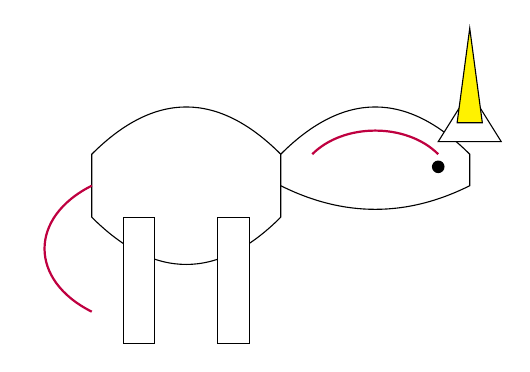
\begin{tikzpicture}[scale=0.8]
  % Body
  \draw[fill=white] (0,0) .. controls (1,1) and (2,1) .. (3,0) -- (3,-1) .. controls (2,-2) and (1,-2) .. (0,-1) -- cycle;
  
  % Legs
  \draw[fill=white] (0.5,-1) -- (0.5,-3) -- (1,-3) -- (1,-1) -- cycle;
  \draw[fill=white] (2,-1) -- (2,-3) -- (2.5,-3) -- (2.5,-1) -- cycle;
  
  % Neck and head
  \draw[fill=white] (3,0) .. controls (4,1) and (5,1) .. (6,0) -- (6,-0.5) .. controls (5,-1) and (4,-1) .. (3,-0.5) -- cycle;
  
  % Ears
  \draw[fill=white] (5.5,0.2) -- (6,1) -- (6.5,0.2) -- cycle;
  
  % Horn
  \draw[fill=yellow] (5.8,0.5) -- (6,2) -- (6.2,0.5) -- cycle;
  
  % Mane
  \draw[thick, color=purple] (3.5,0) .. controls (4,0.5) and (5,0.5) .. (5.5,0);
  
  % Tail
  \draw[thick, color=purple] (0,-0.5) .. controls (-1,-1) and (-1,-2) .. (0,-2.5);
  
  % Eye
  \fill (5.5,-0.2) circle (0.1);
\end{tikzpicture}

\caption{claude-3-opus-20240229} 

\end{figure} 

\begin{figure}[h] 

\centering 

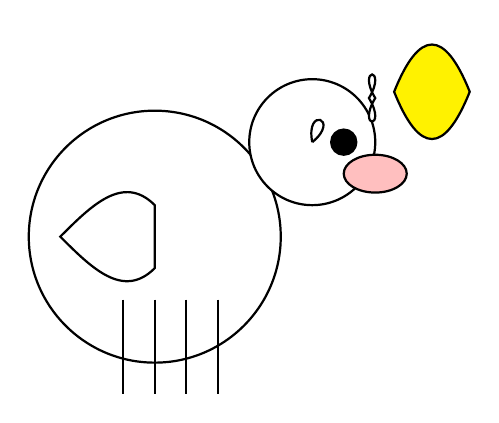
\begin{tikzpicture}[scale=0.8]
    % Body
    \draw[thick, fill=white] (0, 0) circle (2cm);
    
    % Head
    \draw[thick, fill=white] (2.5, 1.5) circle (1cm);
    
    % Ear
    \draw[thick, fill=white] (3.5, 2.2) .. controls (3.2, 2.7) and (3.7, 2.7) .. (3.4, 2.2) .. controls (3.7, 1.7) and (3.2, 1.7) .. (3.5, 2.2) -- cycle;
    
    % Eye
    \draw[thick, fill=black] (3, 1.5) circle (0.2cm);
    
    % Muzzle
    \draw[thick, fill=pink] (3.5, 1) ellipse (0.5cm and 0.3cm);
    
    % Horn
    \draw[thick, fill=yellow] (3.8, 2.3) .. controls (4.2, 3.3) and (4.6, 3.3) .. (5, 2.3) .. controls (4.6, 1.3) and (4.2, 1.3) .. (3.8, 2.3) -- cycle;
    
    % Mane
    \draw[thick, fill=white, rotate around={-20:(2.5, 1.5)}] (2.5, 1.5) .. controls (2.2, 2) and (2.8, 2) .. (2.5, 1.5);
    
    % Legs
    \draw[thick] (0, -1) -- (0, -2.5);
    \draw[thick] (0.5, -1) -- (0.5, -2.5);
    \draw[thick] (-0.5, -1) -- (-0.5, -2.5);
    \draw[thick] (1, -1) -- (1, -2.5);
    
    % Tail
    \draw[thick, fill=white] (0, 0.5) .. controls (-0.5, 1) and (-1, 0.5) .. (-1.5, 0) .. controls (-1, -0.5) and (-0.5, -1) .. (0, -0.5) -- cycle;
\end{tikzpicture}

\caption{claude-3-sonnet-20240229} 

\end{figure} 

\begin{figure}[h] 

\centering 

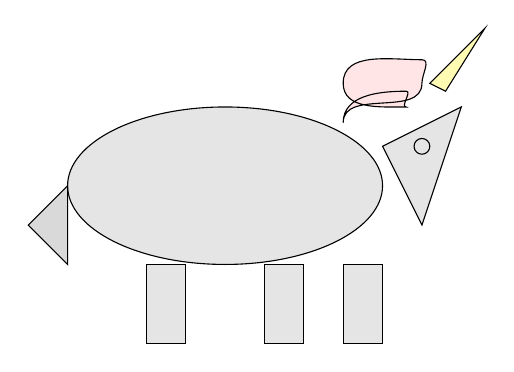
\begin{tikzpicture}
    % Body of the unicorn
    \draw [fill=gray!20] (0,0) ellipse (2 and 1);
    % Legs
    \draw [fill=gray!20] (-1,-1) rectangle (-0.5,-2);
    \draw [fill=gray!20] (0.5,-1) rectangle (1,-2);
    % Tail
    \draw [fill=gray!30] (-2,0) -- (-2.5,-0.5) -- (-2,-1) -- cycle;
    % Head
    \draw [fill=gray!20] (2,0.5) -- (3,1) -- (2.5,-0.5) -- cycle;
    % Eye
    \draw (2.5,0.5) circle (0.1);
    % Horn
    \draw [fill=yellow!30] (2.8,1.2) -- (3.3,2) -- (2.6,1.3) -- cycle;
    % Mane
    \draw[fill=pink!40] (1.5,0.8) to [out=90,in=180] (2.3,1.2) to [out=0,in=180] (2.3,1) to [out=180,in=270] (1.5,1.3) to [out=90,in=180] (2.5,1.6) to [out=0,in=90] (2.5,1.3) to [out=270,in=90] (1.5,0.8);
    % Front leg
    \draw [fill=gray!20] (1.5,-1) rectangle (2,-2);
\end{tikzpicture}

\caption{gpt-4-1106-preview} 

\end{figure} 

\begin{figure}[h] 

\centering 

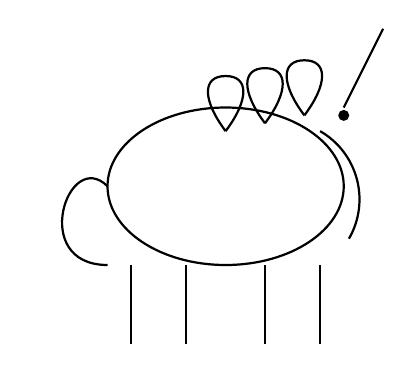
\begin{tikzpicture}
    % Body of the unicorn
    \draw [thick] (0,0) ellipse (1.5 and 1);
    
    % Head of the unicorn
    \draw [thick] (1.2, 0.7) arc (60:-30:1);
    
    % Legs
    \draw [thick] (-0.5,-1) -- (-0.5, -2);
    \draw [thick] (0.5,-1) -- (0.5, -2);
    \draw [thick] (-1.2,-1) -- (-1.2, -2);
    \draw [thick] (1.2,-1) -- (1.2, -2);
    
    % Tail
    \draw [thick] (-1.5,0) .. controls (-2, 0.5) and (-2.5, -1) .. (-1.5, -1);
    
    % Unicorn Horn
    \draw [thick] (1.5, 1) -- (2, 2);
    
    % Eye
    \fill (1.5,0.9) circle (0.07);
    
    % Mane
    \draw [thick] (0.5,0.8) .. controls (0.8, 1.2) and (0.8, 1.5) .. (0.5, 1.5)
                  .. controls (0.2, 1.5) and (0.2, 1.2) .. (0.5, 0.8);
    \draw [thick] (1,0.9) .. controls (1.3, 1.3) and (1.3, 1.6) .. (1, 1.6)
                  .. controls (0.7, 1.6) and (0.7, 1.3) .. (1, 0.9);
    \draw [thick] (0,0.7) .. controls (0.3, 1.1) and (0.3, 1.4) .. (0, 1.4)
                  .. controls (-0.3, 1.4) and (-0.3, 1.1) .. (0, 0.7);
\end{tikzpicture}

\caption{gpt-4-turbo-2024-04-09} 

\end{figure} 

\begin{figure}[h] 

\centering 


\begin{tikzpicture}[scale=0.5]
  % Body
  \fill[white] (0,0) circle (3);
  \fill[gray!20] (0,0) circle (2.5);
  
  % Neck
  \fill[white] (-1.5,2) ellipse (1.5 and 0.75);
  \fill[gray!20] (-1.5,2) ellipse (1.2 and 0.6);
  
  % Head
  \fill[white] (-2.5,3.5) ellipse (1 and 0.6);
  \fill[gray!20] (-2.5,3.5) ellipse (0.8 and 0.5);
  
  % Horn
  \fill[gray!50] (-2.5,4.5) ellipse (0.4 and 0.2);
  
  % Eyes
  \fill[black] (-2.2,3.7) circle (0.1);
  \fill[black] (-2.8,3.7) circle (0.1);
  
  % Mane
  \foreach \x in {-2.5,-2.2,...,0.5}
    \fill[gray!50] (\x,3.8) circle (0.1);
  
  % Legs
  \foreach \x in {-1.5,-0.5,0.5,1.5}
    \fill[gray!20] (\x,-1.5) ellipse (0.5 and 0.3);
  
  % Hooves
  \foreach \x in {-1.5,-0.5,0.5,1.5}
    \fill[black] (\x,-2.2) ellipse (0.3 and 0.2);
\end{tikzpicture}

\caption{llama-3-70b-instruct (1)} 

\end{figure} 

\begin{figure}[h] 

\centering 

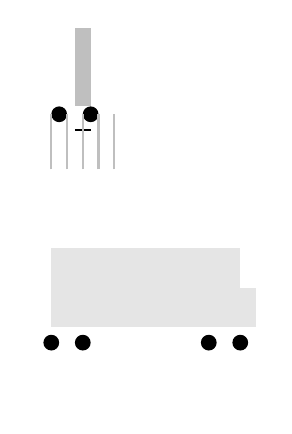
\begin{tikzpicture}
  % Body
  \fill[white] (0,0) circle (1.5);
  \fill[gray!20] (-1.2,0.5) -- (-1.2,-0.5) -- (1.2,-0.5) -- (1.2,0.5) -- cycle;
  
  % Neck
  \fill[white] (-1,0.5) -- (-1,1.5) -- (-0.8,1.5) -- (-0.8,0.5) -- cycle;
  
  % Head
  \fill[white] (-1.2,1.5) -- (-1.2,2.5) -- (-0.6,2.5) -- (-0.6,1.5) -- cycle;
  
  % Horn
  \fill[gray!50] (-0.9,2.3) -- (-0.9,3.3) -- (-0.7,3.3) -- (-0.7,2.3) -- cycle;
  
  % Eyes
  \fill[black] (-1.1,2.2) circle (0.1);
  \fill[black] (-0.7,2.2) circle (0.1);
  
  % Mouth
  \draw[thick] (-0.9,2.0) -- (-0.7,2.0);
  
  % Mane
  \foreach \x in {-1.2,-1.0,...,-0.4} {
    \draw[-,thick,gray!50] (\x,1.5) -- (\x,2.2);
  }
  
  % Legs
  \foreach \x in {-1.2,-0.8,0.8,1.2} {
    \fill[gray!20] (\x,-0.5) -- (\x,0) -- (\x+0.2,0) -- (\x+0.2,-0.5) -- cycle;
  }
  
  % Hooves
  \foreach \x in {-1.2,-0.8,0.8,1.2} {
    \fill[black] (\x,-0.7) circle (0.1);
  }
\end{tikzpicture}

\caption{llama-3-70b-instruct} 

\end{figure} 

\begin{figure}[h] 

\centering 


\begin{tikzpicture}
% Body
\filldraw[fill=white, draw=black] (-3,0) -- (3,0) -- (0,2) -- cycle;

% Horn
\draw[fill=white, draw=black] (0,0) -- (0.5,1) -- (1,0) -- cycle;
\draw[fill=white, draw=black] (0,0) -- (-0.5,1) -- (-1,0) -- cycle;

% Eyes
\filldraw[fill=black, draw=black] (-1.5,0.5) circle (3pt);
\filldraw[fill=black, draw=black] (1.5,0.5) circle (3pt);

% Mane
\draw[thin, fill=white, draw=black] (0,1.5) -- (0.5,2.5) -- (1.5,3.5) -- (0.5,2.5) -- cycle;
\draw[thin, fill=white, draw=black] (0,1.5) -- (-0.5,2.5) -- (-1.5,3.5) -- (-0.5,2.5) -- cycle;

% Tail
\draw[thin, fill=white, draw=black] (0,0) -- (0,-2);
\end{tikzpicture}


\caption{llama-3-8b-instruct (1)} 

\end{figure} 

\begin{figure}[h] 

\centering 


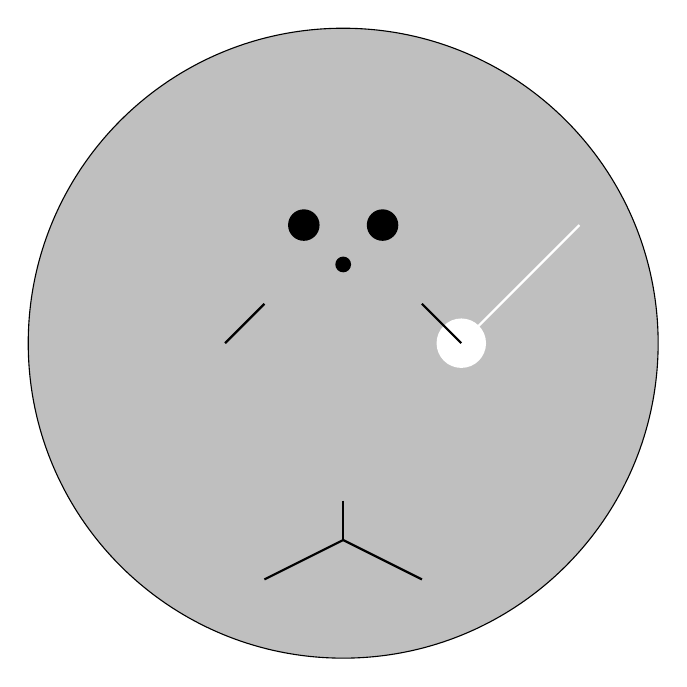
\begin{tikzpicture}
% Body
\draw [fill=lightgray] (0,0) circle (4cm);

% Horn
\draw [thick, white] (1.5,0) -- (3,1.5);
\draw [thick, white, fill=white] (1.5,0) circle (0.3cm);

% Ears
\draw [thick] (-1.5,0) -- (-1,0.5);
\draw [thick] (1.5,0) -- (1,0.5);

% Eyes and nose
\fill [black] (0.5,1.5) circle (0.2cm);
\fill [black] (-0.5,1.5) circle (0.2cm);
\fill [black] (0,1) circle (0.1cm);

% Tail
\draw [thick] (0,-2) -- (0,-2.5);

% Legs
\draw [thick] (0,-2.5) -- (-1,-3);
\draw [thick] (0,-2.5) -- (1,-3);

\end{tikzpicture}

\caption{llama-3-8b-instruct (2)} 

\end{figure} 

\begin{figure}[h] 

\centering 

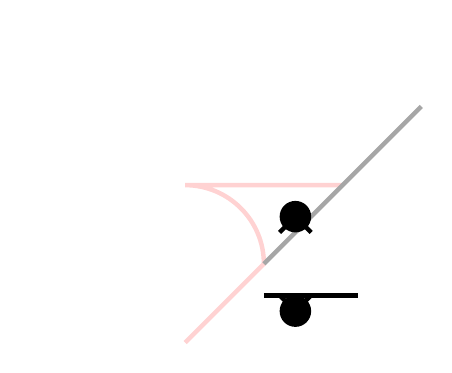
\begin{tikzpicture}[scale=2]

% Define the colors
\colorlet{unicornwhite}{white}
\colorlet{unicornblue}{gray!70}
\colorlet{unicornpink}{pink!70}

% Draw the body
\fill[unicornwhite] (0,0) -- (1,1) arc (0:180:1) -- cycle;

% Draw the mane
\draw[ultra thick, unicornpink] (0,0) -- (0.5,0.5) arc (0:90:0.5) -- (1,1);

% Draw the horn
\draw[ultra thick, unicornblue] (0.5,0.5) -- (1.5,1.5);

% Draw the eyes
\fill[black] (0.7,0.8) circle (0.1);
\fill[black] (0.7,0.2) circle (0.1);

% Draw the eyelashes
\draw[ultra thick, black] (0.7,0.8) -- (0.8,0.7);
\draw[ultra thick, black] (0.7,0.8) -- (0.6,0.7);
\draw[ultra thick, black] (0.7,0.2) -- (0.8,0.3);
\draw[ultra thick, black] (0.7,0.2) -- (0.6,0.3);

% Draw the mouth
\draw[ultra thick, black] (0.5,0.3) -- (1.1,0.3);

\end{tikzpicture}

\caption{llama-3-8b-instruct (3)} 

\end{figure} 

\begin{figure}[h] 

\centering 


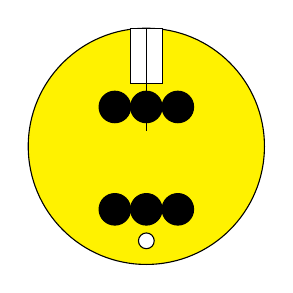
\begin{tikzpicture}
\draw[fill=yellow] (0,0) circle (1.5) node (head) {};
\draw[fill=black] (0,0.5) circle (0.2);
\draw[fill=black] (0.4,0.5) circle (0.2);
\draw[fill=black] (-0.4,0.5) circle (0.2);
\draw[fill=black] (0,-0.8) circle (0.2);
\draw[fill=black] (0.4,-0.8) circle (0.2);
\draw[fill=black] (-0.4,-0.8) circle (0.2);
\draw (0,0.6) -- (0,1.1) node (ear) {};
\draw (0,0.6) -- (0,0.2) node (ear2) {};
\draw[fill=white] (0,1.2) circle (0.1) node (horn) {};
\draw[fill=white] (0,-1.2) circle (0.1) node (horn2) {};
\draw[fill=white] (0,0.8) -- (0.2,0.8) -- (0.2,1.5) -- (0,1.5) -- cycle;
\draw[fill=white] (0,0.8) -- (-0.2,0.8) -- (-0.2,1.5) -- (0,1.5) -- cycle;
\end{tikzpicture}

\caption{llama-3-8b-instruct (4)} 

\end{figure} 

\begin{figure}[h] 

\centering 

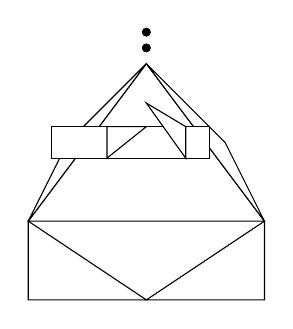
\begin{tikzpicture}
  % Body
  \draw[fill=white] (-1.5,0) -- (1.5,0) -- (0,2) -- cycle;
  \draw[fill=white] (-1.5,0) -- (0,2) -- (-1,1) -- cycle;
  \draw[fill=white] (1.5,0) -- (0,2) -- (1,1) -- cycle;

  % Horn
  \draw[fill=white] (-1.2,1.2) -- (0.8,1.2) -- (0.8,0.8) -- (-1.2,0.8) -- cycle;

  % Eyes
  \draw[fill=black] (0,2.2) circle (0.05);
  \draw[fill=black] (0,2.4) circle (0.05);

  % Mane
  \draw[fill=white] (0,1.5) -- (0.5,1.2) -- (0.5,0.8) -- cycle;
  \draw[fill=white] (0,1.2) -- (-0.5,1.2) -- (-0.5,0.8) -- cycle;

  % Legs
  \draw[fill=white] (1.5,0) -- (1.5,-1) -- (0,-1) -- cycle;
  \draw[fill=white] (-1.5,0) -- (-1.5,-1) -- (0,-1) -- cycle;
\end{tikzpicture}

\caption{llama-3-8b-instruct} 

\end{figure} 

\begin{figure}[h] 

\centering 


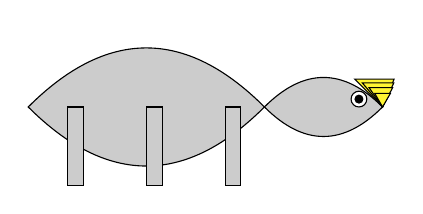
\begin{tikzpicture}
% Unicorn body
\draw[fill=gray!40] (0,0) .. controls (1,1) and (2,1) .. (3,0) .. controls (2,-1) and (1,-1) .. (0,0) -- cycle;

% Unicorn head
\draw[fill=gray!40] (3,0) .. controls (3.5,0.5) and (4,0.5) .. (4.5,0) .. controls (4,-0.5) and (3.5,-0.5) .. (3,0) -- cycle;

% Unicorn eye
\filldraw[fill=white] (4.2,0.1) circle (0.1);
\filldraw[fill=black] (4.2,0.1) circle (0.05);

% Unicorn horn
\draw[fill=yellow!80] (4.5,0) -- ++(135:0.5) -- ++(0.5,0) -- cycle;
\draw[fill=yellow!80] (4.5,0) -- ++(130:0.4) -- ++(0.4,0) -- cycle;
\draw[fill=yellow!80] (4.5,0) -- ++(125:0.3) -- ++(0.3,0) -- cycle;
\draw[fill=yellow!80] (4.5,0) -- ++(120:0.2) -- ++(0.2,0) -- cycle;

% Unicorn legs
\draw[fill=gray!40] (0.5,0) rectangle (0.7,-1);
\draw[fill=gray!40] (1.5,0) rectangle (1.7,-1);
\draw[fill=gray!40] (2.5,0) rectangle (2.7,-1);
\end{tikzpicture}

\caption{mixtral-8x22b-instruct-v0.1 (1)} 

\end{figure} 

\begin{figure}[h] 

\centering 

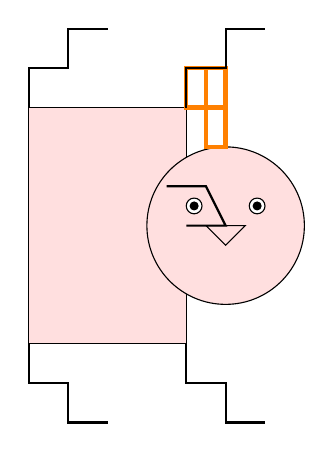
\begin{tikzpicture}[scale=0.5]
% Body
\filldraw[fill=pink!50!white, draw=black] (0,0) rectangle (4,6);
% Head
\filldraw[fill=pink!50!white, draw=black] (5,3) circle (2cm);
% Eyes
\filldraw[fill=white, draw=black] (5.8,3.5) circle (0.2cm);
\filldraw[fill=white, draw=black] (4.2,3.5) circle (0.2cm);
% Pupils
\filldraw[fill=black, draw=black] (5.8,3.5) circle (0.1cm);
\filldraw[fill=black, draw=black] (4.2,3.5) circle (0.1cm);
% Nose
\filldraw[fill=pink!50!white, draw=black] (5,2.5) -- (5.5,3) -- (4.5,3) -- cycle;
% Horn
\draw[ultra thick, draw=orange] (5,5) -- ++(0,2) -- ++(-1,0) -- ++(0,-1) -- ++(1,0) -- ++(0,1) -- ++(-0.5,0) -- ++(0,-2) -- cycle;
% Legs
\draw[thick, draw=black] (0,0) -- ++(0,-1) -- ++(1,0) -- ++(0,-1) -- ++(1,0);
\draw[thick, draw=black] (4,0) -- ++(0,-1) -- ++(1,0) -- ++(0,-1) -- ++(1,0);
\draw[thick, draw=black] (0,6) -- ++(0,1) -- ++(1,0) -- ++(0,1) -- ++(1,0);
\draw[thick, draw=black] (4,6) -- ++(0,1) -- ++(1,0) -- ++(0,1) -- ++(1,0);
% Tail
\draw[thick, draw=black] (4,3) -- ++(1,0) -- ++(-0.5,1) -- ++(-1,0);
\end{tikzpicture}

\caption{mixtral-8x22b-instruct-v0.1 (2)} 

\end{figure} 

\begin{figure}[h] 

\centering 

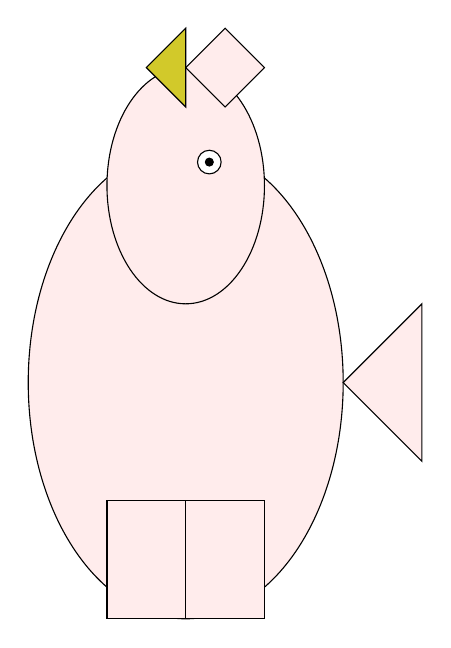
\begin{tikzpicture}

% Body
\filldraw[fill=pink!30!white,draw=black] (0,0) ellipse (2 and 3);

% Head
\filldraw[fill=pink!30!white,draw=black] (0,2.5) ellipse (1 and 1.5);

% Ear
\filldraw[fill=pink!30!white,draw=black] (0.5,3.5) -- (1,4) -- (0.5,4.5) -- (0,4) -- cycle;

% Eye
\filldraw[fill=white,draw=black] (0.3,2.8) circle (0.15);
\filldraw[fill=black,draw=black] (0.3,2.8) circle (0.05);

% Horn
\draw[fill=yellow!80!black,draw=black] (0,3.5) -- (0,4.5) -- (-0.5,4) -- cycle;

% Legs
\filldraw[fill=pink!30!white,draw=black] (-1,-1.5) -- (-1,-3) -- (0,-3) -- (0,-1.5) -- cycle;
\filldraw[fill=pink!30!white,draw=black] (1,-1.5) -- (1,-3) -- (0,-3) -- (0,-1.5) -- cycle;

% Tail
\draw[fill=pink!30!white,draw=black] (2,0) -- (3,-1) -- (3,1) -- cycle;

\end{tikzpicture}

\caption{mixtral-8x22b-instruct-v0.1} 

\end{figure} 

\begin{figure}[h] 

\centering 

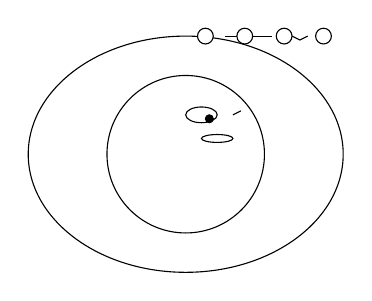
\begin{tikzpicture}
    % Body
    \draw[fill=white] (0,0) ellipse (2cm and 1.5cm);
    % Head
    \draw[fill=white] (0,0) ellipse (1cm and 1cm);
    \draw[fill=white] (0.2,0.5) ellipse (0.2cm and 0.1cm);
    \draw[fill=white] (0.4,0.2) ellipse (0.2cm and 0.05cm);
    % Eye
    \draw[fill=black] (0.3,0.45) circle (0.05cm);
    % Horn
    \draw[fill=white] (0.6,0.5) -- (0.7,0.55);
    % Legs
    \draw[fill=white] (0.25,1.5) -- (0.35,1.5);
    \draw[fill=white] (0.55,1.5) -- (0.65,1.5);
    \draw[fill=white] (0.85,1.5) -- (0.95,1.5);
    \draw[fill=white] (1.15,1.5) -- (1.25,1.5);
    % Tail
    \draw[fill=white] (1.35,1.5) -- (1.45,1.45) -- (1.55,1.5);
    % Mane
    \draw[fill=white] (0.5,1.5) -- (0.7,1.5);
    \draw[fill=white] (0.7,1.5) -- (0.9,1.5);
    \draw[fill=white] (0.9,1.5) -- (1.1,1.5);
    % Hooves
    \draw[fill=white] (0.25,1.5) circle (0.1cm);
    \draw[fill=white] (0.75,1.5) circle (0.1cm);
    \draw[fill=white] (1.25,1.5) circle (0.1cm);
    \draw[fill=white] (1.75,1.5) circle (0.1cm);
\end{tikzpicture}

\caption{phi-3-mini-128k-instruct (1)} 

\end{figure} 

\begin{figure}[h] 

\centering 

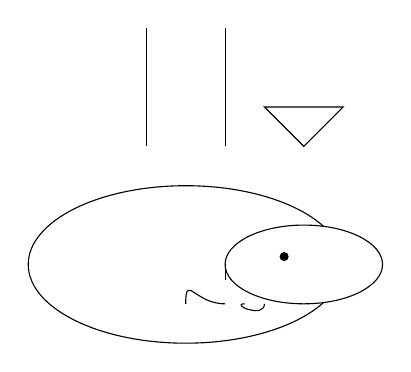
\begin{tikzpicture}
    % Body
    \draw[fill=white] (0,0) ellipse (2cm and 1cm);
    % Head
    \draw[fill=white] (1.5,0) ellipse (1cm and 0.5cm);
    % Eye
    \draw[fill=black] (1.25,0.1) circle (0.05cm);
    % Mane
    \draw[fill=white] (0,-0.5) to[out=90,in=180,looseness=2] (0.5,-0.5);
    \draw[fill=white] (0.75,-0.5) to[out=180,in=270,looseness=2] (1,-0.5);
    % Horn
    \draw[fill=white] (0.5,0) -- (0.5,-0.2);
    % Legs
    \draw[fill=white] (-0.5,1.5) -- (-0.5,2) -- (-0.5,2.5) -- (-0.5,3);
    \draw[fill=white] (0.5,1.5) -- (0.5,2) -- (0.5,2.5) -- (0.5,3);
    % Tail
    \draw[fill=white] (1,2) -- (1.5,1.5) -- (2,2) -- cycle;
\end{tikzpicture}

\caption{phi-3-mini-128k-instruct} 

\end{figure} 

\end{document}

